%\clearpage
%\section{Logaritmische vergelijkingen}
%
%Een vergelijking noemen we logaritmisch als de \emph{onbekende voorkomt in het
%argument van een logaritme}. Omdat een logaritme alleen
%gedefinieerd is als het argument positief is, zijn er
%bestaansvoorwaarden: niet alle waarden van de onbekende zijn toegelaten. 
%Het is belangrijk dat je de gevonden oplossingen als laatste nog eens toetst aan de bestaansvoorwaarden. Dit wordt duidelijk in voorbeeld 3. 
%
%
%De algemene oplossingsmethode voor een logaritmische vergelijking is:
%\begin{enumerate}
%\item Noteer de bestaansvoorwaarden.
%    \item  Gebruik de rekenregels van de logaritmen (\cref{tbl:logexpverband}) om beide leden van de vergelijking te
%schrijven als \'{e}\'{e}n logaritme met hetzelfde grondtal, of als  een
%getal.
%
%    \item  Zo ontstaan er 2 mogelijke vormen:
%\begin{enumerate}
%    \item  $ \log_{g}(f(x))=\log_{g}(h(x))$: Omdat  de logaritmische functie een ��n-op-��n relatie is 
%    volgt dat  $f(x)=h(x)$. Dit is meestal een vergelijking zonder logaritme of exponent en kunnen we dus oplossen.
%    \item  $\log_{g}(f(x))=b$: De logaritme werken we weg door de
%    definitie van de logaritme toe te passen. We bekomen de vergelijking
%    $g^{b}=f(x)$.
%\end{enumerate}
%\item Toets de gevonden oplossing aan de bestaansvoorwaarden.
%\end{enumerate}
%
%
%\subsection{Voorbeeld 1}
%\begin{equation}
%\log(x+3)=\log(5) + \log\left(\frac{1}{3}\right)
%\label{logvgl:vb1}
%\end{equation}
%
%\begin{enumerate}
%    \item  Bestaansvoorwaarden
%    \[x+3> 0 \quad \Leftrightarrow \quad
%    x>-3
%    \]
%
%    \item  Met behulp van de rekenregels schrijven we in het rechterlid de som van de logaritmen als de logaritme van een product:
%	\[
%        \log(x+3)=\log\left(5\cdot \frac{1}{3}\right)
%        \]
%        \item Bij puntje 3 van de algemene oplossingsmethode bekomen we vorm (a). Als de $\log(a)=\log(b)$, moet $a=b$ (��n-op-��n relatie):
%\[
%    x+3=\frac{5}{3} 
%    \]
%    Deze vergelijking kunnen we eenvoudig oplossen:
%    \[  x=-\frac{4}{3}
%	\]
%    \item   We toetsen de gevonden oplossing aan de bestaansvoorwaarde: $-4/3$ is inderdaad groter dan $3$.
%\end{enumerate}
% De oplossing voor vergelijking~(\ref{logvgl:vb1}) is $x=-4/3$. 
%
%\subsection{Voorbeeld 2}
%\begin{equation}
%   \log_{\frac13}(2x-1)=-1
%   \label{logvgl:vb2}
%\end{equation}
%\begin{enumerate}
%    \item  Bestaansvoorwaarden 
%    \[
%   2x-1>0  \quad \Leftrightarrow 
%    \quad  x>-\frac12
%    \]
%   \item Het linkerlid is een logaritme; het rechterlid is een getal.
%    \item  In puntje 3 van de algemene oplossingsmethode hebben we vorm (b). We passen de definitie van de logaritme toe.
%    \begin{align*}
%        \left(\frac{1}{3}\right)^{-1}&=2 x-1 \\
%        &\Updownarrow\\
%         3&=2x -1\\
%        &\Updownarrow\\
%    x&=2
%    \end{align*}
%
%    \item  De gevonden oplossing  $x=2$ voldoet aan de
%    bestaansvoorwaarde. 
%\end{enumerate}
% De oplossing voor vergelijking~(\ref{logvgl:vb2}) is $x=2$. 
%
%Op \cref{fig: fig_log_vgl_vb2} wordt de oplossing van vergelijking~(\ref{logvgl:vb2}) getoond als snijpunt van de functies $f(x)=\log_{\frac13}(2x-1)$ en $g(x)=-1$.
%\begin{figure}[htbp]
%    \centering
%           \begin{tikzpicture}[line cap=round,line join=round,x=1.4cm,y=1.4cm]
%\draw[->] (-1.2,0) -- (5.5,0) node [at end, below] {$x$};
%\foreach \x in {-1,1,2,...,5}
%\draw[shift={(\x,0)}] (0pt,2pt) -- (0pt,-2pt) node[below] {\footnotesize $\x$};
%\draw[->] (0,-2.1) -- (0,2.3) node [at end, left] {$y$};
%\foreach \y in {-2,-1,1,2}
%\draw[shift={(0,\y)},color=black] (2pt,0pt) -- (-2pt,0pt) node[left] {\footnotesize $\y$};
%\node[below left] (0,0) {\footnotesize 0};
%\draw [domain=0.6:5,samples=80,thick,blue] plot(\x,{ln(2*\x-1)/ln(1/3))}); 
%\draw[blue] (1.5,1.8) node {$f(x)=\log_{\frac{1}{3}}(2x-1)$};
%\draw [thick,red] (-1,-1) -- (5,-1) ;
%\draw[red] (4.5,-0.8) node {$g(x)=-1$};
%\draw[dashed] (2,0) -- (2,-1);
%    \filldraw [] (2,-1) circle (2pt) node[below left] { $(\num{2};\num{-1})$};
%\end{tikzpicture}
%    \caption{Snijpunt van de functies $f(x)=\log_{\frac13}(2x-1)$ en $g(x)=-1$}
%    \label{fig: fig_log_vgl_vb2}
%\end{figure}
%
%\subsection{Voorbeeld 3}
%\begin{equation}
%   \log_5(3x-5)=\log_5(x^2+4x-11)
%   \label{logvgl:vb3}
%\end{equation}
%\begin{enumerate}
%    \item  Bestaansvoorwaarden 
%    \begin{align*}
%   3x-5>0  \quad &\text{en} 
%    \quad   x^2+4x-11>0\\
%   & \Updownarrow\\
%   x>\frac53 \quad &\text{en} \quad x<\num{-5.8}~\text{ of }~x>\num{1.87}
%    \end{align*}
%   \item Zowel het linker-als het rechterlid zijn een logaritme met hetzelfde grondtal.
%   
%   \item De logaritmische functie is een ��n-op-��n relatie zodat 
%   \begin{align*}
%   3x-5&=x^2+4x-11\\
%   &\Updownarrow \\
%   x^2+x-6&=0 \\
%   &\Updownarrow \\
%x=-3\quad&\text{of}\quad x=2
%   \end{align*}
%   \item Enkel de oplossing $x=2$ voldoet aan de bestaansvoorwaarden.
%\end{enumerate}
%De oplossing voor vergelijking~(\ref{logvgl:vb3}) is $x=2$.
%
%%Op \cref{fig: fig_log_vgl_vb3} wordt de oplossing van vergelijking~(\ref{logvgl:vb3}) getoond als snijpunt van de functies $f(x)= \log_5(3x-5)$ en $g(x)=\log_5(x^2+4x-11)$.
%\begin{figure}[htbp]
%    \centering
%    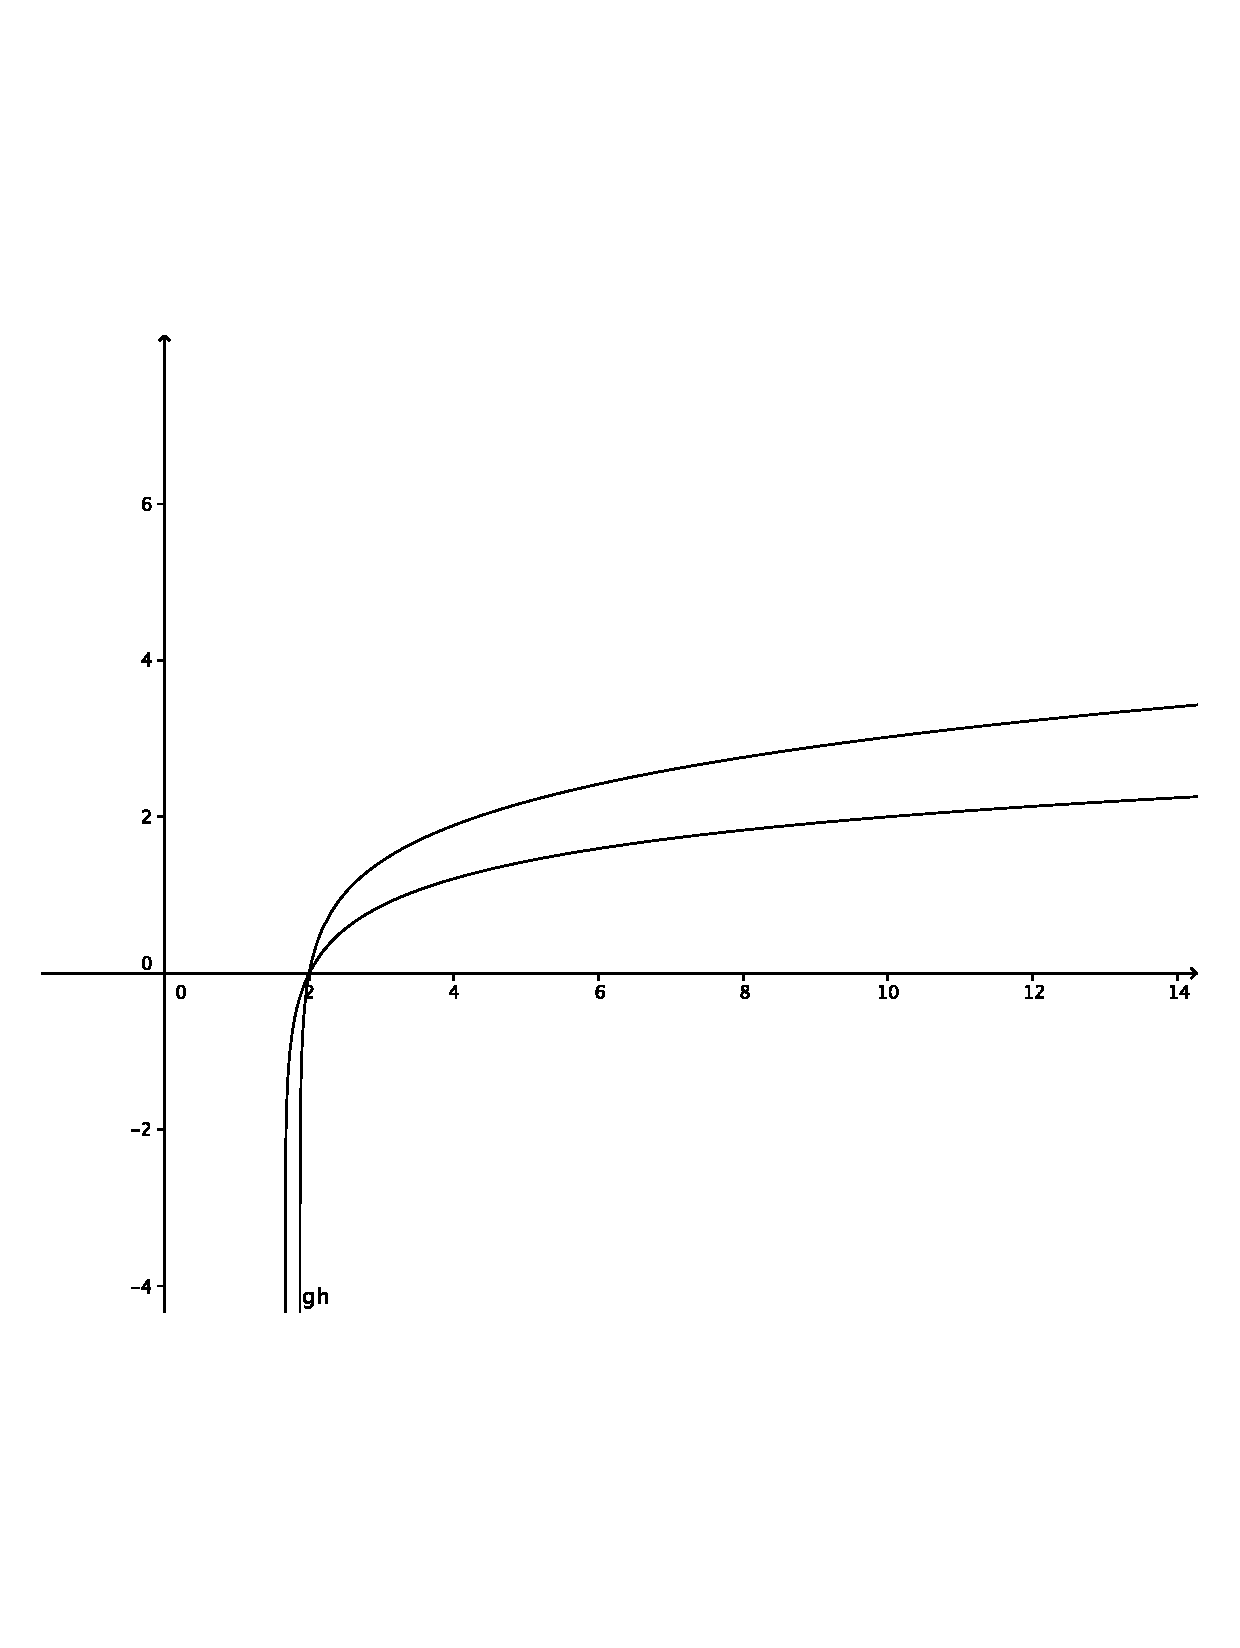
\includegraphics[width=10.7cm]{figuren/euler_expfuncties/fig_log_vgl_vb3.pdf}
%    \caption{Snijpunt van de functies $f(x)= \log_5(3x-5)$ en $g(x)=\log_5(x^2+4x-11)$}
%    \label{fig: fig_log_vgl_vb3}
%%\end{figure}
